\documentclass{article}
\usepackage{../../Self_Style}

\title{Math CS 121 HW 8}
\author{Zih-Yu Hsieh}
\date{\today}

\begin{document}
\maketitle

\section*{1}
\begin{ques}\label{q1}
    8.3.7:

    Let $X$ and $Y$ be continuous random variables with joint probability density function given by 
    $$f(x,y)=\begin{cases}
        e^{-x(y+1)} & x\geq 0,\ 0\leq y\leq e-1\\
        0 & \text{elsewhere}
    \end{cases}$$
    Calculate $\EE[X|Y=y]$.
\end{ques}

\begin{proof}
    First, we'll gather the marginal density of $Y$: If $t<0$ or $t>e-1$, since $f(x,t)=0$, then $f_y(t) = int_{0}^{\infty}f(x,t)dx = 0$; else, if $t in [0,e-1]$, $f_y(t)$ is given as follow:
    \begin{align}
        f_y(t)=\int_{0}^{\infty}f(x,t)dx = \int_{0}^{\infty}e^{-x(t+1)}dx = \frac{-1}{t+1}e^{-x(t+1)}\bigg|_{0}^{\infty} = \frac{1}{t+1}
    \end{align} 
    So, $f_y(t) = \begin{cases}
        \frac{1}{t+1} & 0\leq t\leq e-1\\ 0 & \text{otherwise}
    \end{cases}$. 

    This indicates that the conditional probability density $f_{X|Y}(s|t)$ is only defined for $t \in [0,e-1]$ (since it requires $f_y(t)\neq 0$ on the region). Which, one has the following:
    \begin{align}
        t\in[0,e-1],\quad f_{X|Y}(s|t) = \frac{f(s,t)}{f_y(t)} \begin{cases}
            (t+1)e^{-s(t+1)} & s\geq 0\\
            0 & \text{otherwise}
        \end{cases}
    \end{align}
    Hence, given $Y=y$ (where $y in [0,e-1]$), the expectation of $X$ is given as follow:
    \begin{align}
        \EE[X|Y=y] &= \int_{0}^{\infty}x \cdot f_{X|Y}(x|y)dx = \int_{0}^{\infty}x(y+1)e^{-x(y+1)}dx = -xe^{-x(y+1)}\bigg|_{0}^{\infty} + \int_{0}^{\infty}e^{-x(y+1)}dx\\
        &= -\frac{1}{y+1}e^{-x(y+1)}\bigg|_{0}^{\infty} = \frac{1}{y+1}
    \end{align}
\end{proof}

\newpage

\section*{2}
\begin{ques}\label{q2}
    8.3.18:

    Let $X$ and $Y$ be continuous random variables with joint probaility density function 
    $$f(x,y) = \begin{cases}
        n(n-1)(y-x)^{n-2} & 0\leq x\leq y\leq 1\\
        0 &\text{otherwise}
    \end{cases}$$
    Find the conditional expectation of $Y$ given that $X=x$.
\end{ques}

\begin{proof}
    First, we'll calculate the marginal density of $X$ (xhere $X,Y in [0,1]$): Given $x<0$ or $x>1$, since $f(x,y)=0$, then $f_X(t) = \int_{0}^{1}f(t,y) dy =0$. Else, if $0\leq x\leq 1$, it's described as follow (Note: if $t>y$, then $f(t,y)=0$):
    \begin{align}
        f_X(t) = \int_{0}^{1}f(t,y) dy = \int_{t}^{1}n(n-1)(y-t)^{n-2}dy = n(y-t)^{n-1}\bigg|_{0}^{1} = n\left((1-t)^{n-1}-(-t)^{n-1}\right)
    \end{align}
    As a result, the conditional density $f_{Y|X}(s|t) = \frac{f(t,s)}{f_X(t)}$ is only defined on some subset of $t\in [0,1]$. Which, fixing $X=x$ (or $t=x$), the conditional expectation of $Y$ is given as follow:
    \begin{align}
        \EE[Y|X=x] &= \int_{0}^{1}y\cdot f_{Y|X}(y|x)dy  = \int_{x}^{1}y\cdot\frac{n(n-1)(y-x)^{n-2}}{n\left((1-x)^{n-1}-(-x)^{n-1}\right)}dy\\
        &= y\cdot \frac{(y-x)^{n-1}}{\left((1-x)^{n-1}-(-x)^{n-1}\right)}\bigg|_{x}^{1} - \int_{x}^{1}\frac{(y-x)^{n-1}}{\left((1-x)^{n-1}-(-x)^{n-1}\right)}dy \\
        &= \frac{(1-x)^{n-1}}{\left((1-x)^{n-1}-(-x)^{n-1}\right)} - \frac{(y-x)^n}{n\left((1-x)^{n-1}-(-x)^{n-1}\right)}\bigg|_{x}^{1}\\
        &= \frac{(1-x)^{n-1}}{\left((1-x)^{n-1}-(-x)^{n-1}\right)} - \frac{(1-x)^n}{n\left((1-x)^{n-1}-(-x)^{n-1}\right)}
    \end{align}
\end{proof}

\newpage

\section*{3}
\begin{ques}\label{q3}
    8.4.8:

    Prove that if $X$ and $Y$ are independent standard normal random variables, then $X+Y$ and $X-Y$ are independent random variables. This is a special case of the following important theorem:
    \begin{thm}
        Let $X$ and $Y$ be independent random variables with a common distribution $F$. The random variables $X+Y$ and $X-Y$ are independent if and only if $F$ is a normal distribution function.
    \end{thm}
\end{ques}

\begin{proof}
    Given $X,Y \sim N(0,1)$, then one has $f_X(t)=f_Y(t) = \frac{1}{\sqrt{2\pi}}e^{-x^2/2}$. To show that $U=X+Y, V=X-Y$ are independent, we'll verify that the joint probability density of $U,V$ is separable. 

    \hfil

    First, since $-Y\sim N(0,1)$ (due to the fact that the probability density $f_Y(t)$ is symmetric about $x$-axis, so one has $\PP(-Y\leq t) = \PP(Y\geq -t) = \int_{-t}^{\infty}f_Y(t)dt = \int_{-\infty}^{t}f_Y(t)dt = \PP(Y\leq t)$), so based on the additivity of normal distribution, one has $U=X+Y\sim N(0+0,1+1) = N(0,2)$, and $V=X-Y\sim N(0+0,1+1) = N(0,2)$ also (with mean $\mu=0$, and variance $\sigma^2=2$, or standard deviation $\sigma=\sqrt{2}$). Hence, one has $f_U(s) = f_V(s) = \frac{1}{\sqrt{2}\cdot \sqrt{2\pi}}e^{-(s/\sqrt{2})^2/2}$.

    \hfil

    Given the definition of $U,V$, one can retrieve $X = \frac{U+V}{2}$, and $Y = \frac{U-V}{2}$. So, given this transformation $(X,Y) = T(U,V)$, one has the differential and Jacobian determinant given as follow:
    \begin{align}
        dT = \begin{pmatrix}
            \frac{\partial x}{\partial u} & \frac{\partial x}{\partial v}\\ \frac{\partial y}{\partial u} & \frac{\partial y}{\partial v}
        \end{pmatrix} = \frac{1}{2}\begin{pmatrix}
            1&1\\1&-1
        \end{pmatrix} \implies |\det J| = \frac{1}{2}
    \end{align}
    Hence, with $f_{X,Y}(x,y) = f_X(x)f_Y(y)$ (based on their independence), one has the joint probability density $f_{U,V}(u,v)$ being as follow:
    \begin{align}
        f_{U,V}(u,v) &= f_{X,Y}(x,y)|\det J| = \frac{1}{2}f_{X,Y}\left(\frac{u+v}{2},\frac{u-v}{2}\right) = \frac{1}{4\pi}\exp\left(-\frac{1}{2}\left(\frac{u+v}{2}\right)^2\right)\exp\left(-\frac{1}{2}\left(\frac{u-v}{2}\right)^2\right)\\
        &= \frac{1}{4\pi}\exp\left(-\frac{(u^2+v^2+2uv)+(u^2+v^2-2uv)}{8}\right) = \frac{1}{4\pi}e^{-u^2/4}e^{-v^2/4} \\
        &= \left(\frac{1}{\sqrt{2}\cdot\sqrt{2\pi}}e^{-\frac{(u/\sqrt{2})^2}{2}}\right)\left(\frac{1}{\sqrt{2}\cdot\sqrt{2\pi}}e^{-(v/\sqrt{2})^2/2}\right) = f_U(u)f_V(v)
    \end{align}
    Since the probability density is separable (with $f_{U,V}(u,v) = f_U(u)f_V(v)$), one can conclude that $U=X+Y,V=X-Y$ are independent.
\end{proof}

\newpage

\section*{4}
\begin{ques}\label{q4}
    8.Rev.16:

    A point is selected at random from the bounded region between the curves $y=x^2-1$ and $y=1-x^2$. Let $X$ be the $x$-coordinate, and let $Y$ be the $y$-coordinate of the point selected. Determine if $X$ and $Y$ are independent.
\end{ques}

\begin{proof}
    In case to show that they're not independent, we aim to show there exists $a,b$, such that $\PP(Y\leq b|X\leq a)\neq \PP(Y\leq b)$ (Which, the probability can be intepreted as the proportion of the area, if it's measurable set).

    Given the area bounded by $x^2-1$ and $1-x^2$, it's given by the area on $-1\leq x\leq 1$ ($x=\pm 1$ is where the two equations meet), with the relation $x^2-1\leq y\leq 1-x^2$ (after solving the inequality).

    \hfil

    Consider $b=\frac{3}{4}$ and $a=-\frac{1}{2}$: Suppose the point $(x,y)$ satisfies $x\leq a=-\frac{1}{2}$, then one has $y \leq 1-x^2 \leq 1-\frac{1}{4}=\frac{3}{4}$, so $\PP(Y\leq \frac{3}{4}|X\leq -\frac{1}{2}) = 1$ (since if $x\leq -\frac{1}{2}$, $y\leq \frac{3}{4}$ is guaranteed). Pictorially, we have the following graph as the region:
    \begin{figure}[h!]
        \centering
        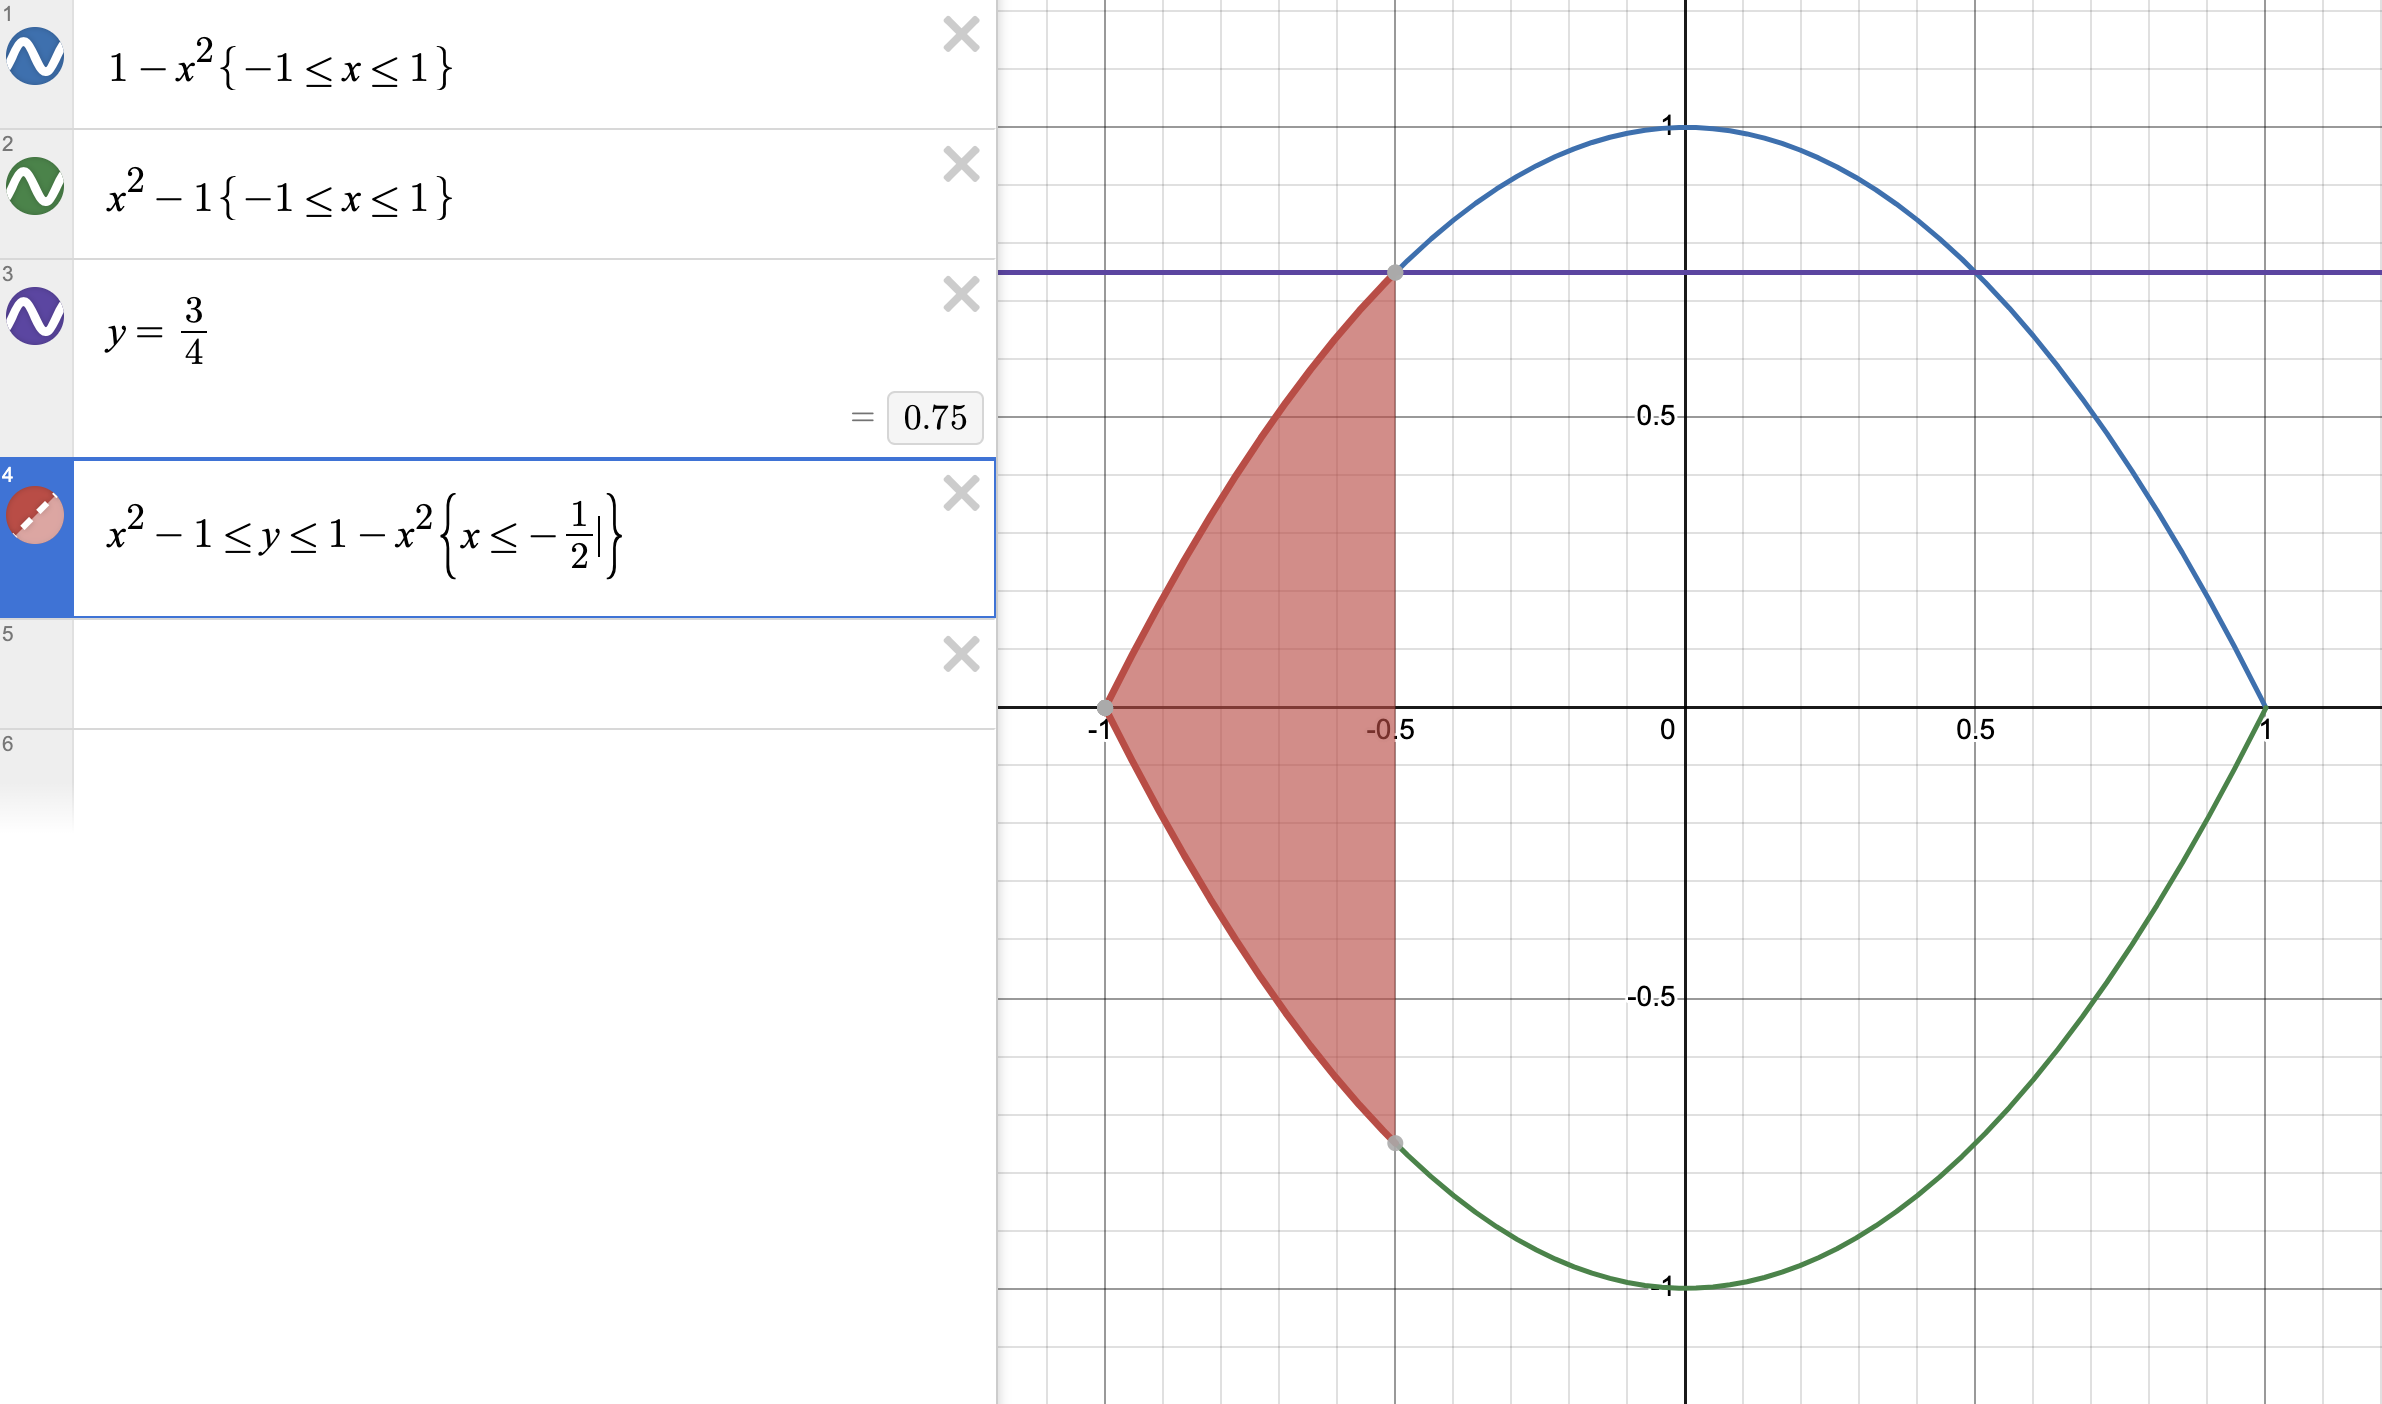
\includegraphics[width=110mm]{q4_g1.png}
    \end{figure}


    However, if consider the probabilty $\PP(Y\leq \frac{3}{4})$, it's considering the following region:
    \begin{figure}[h!]
        \centering
        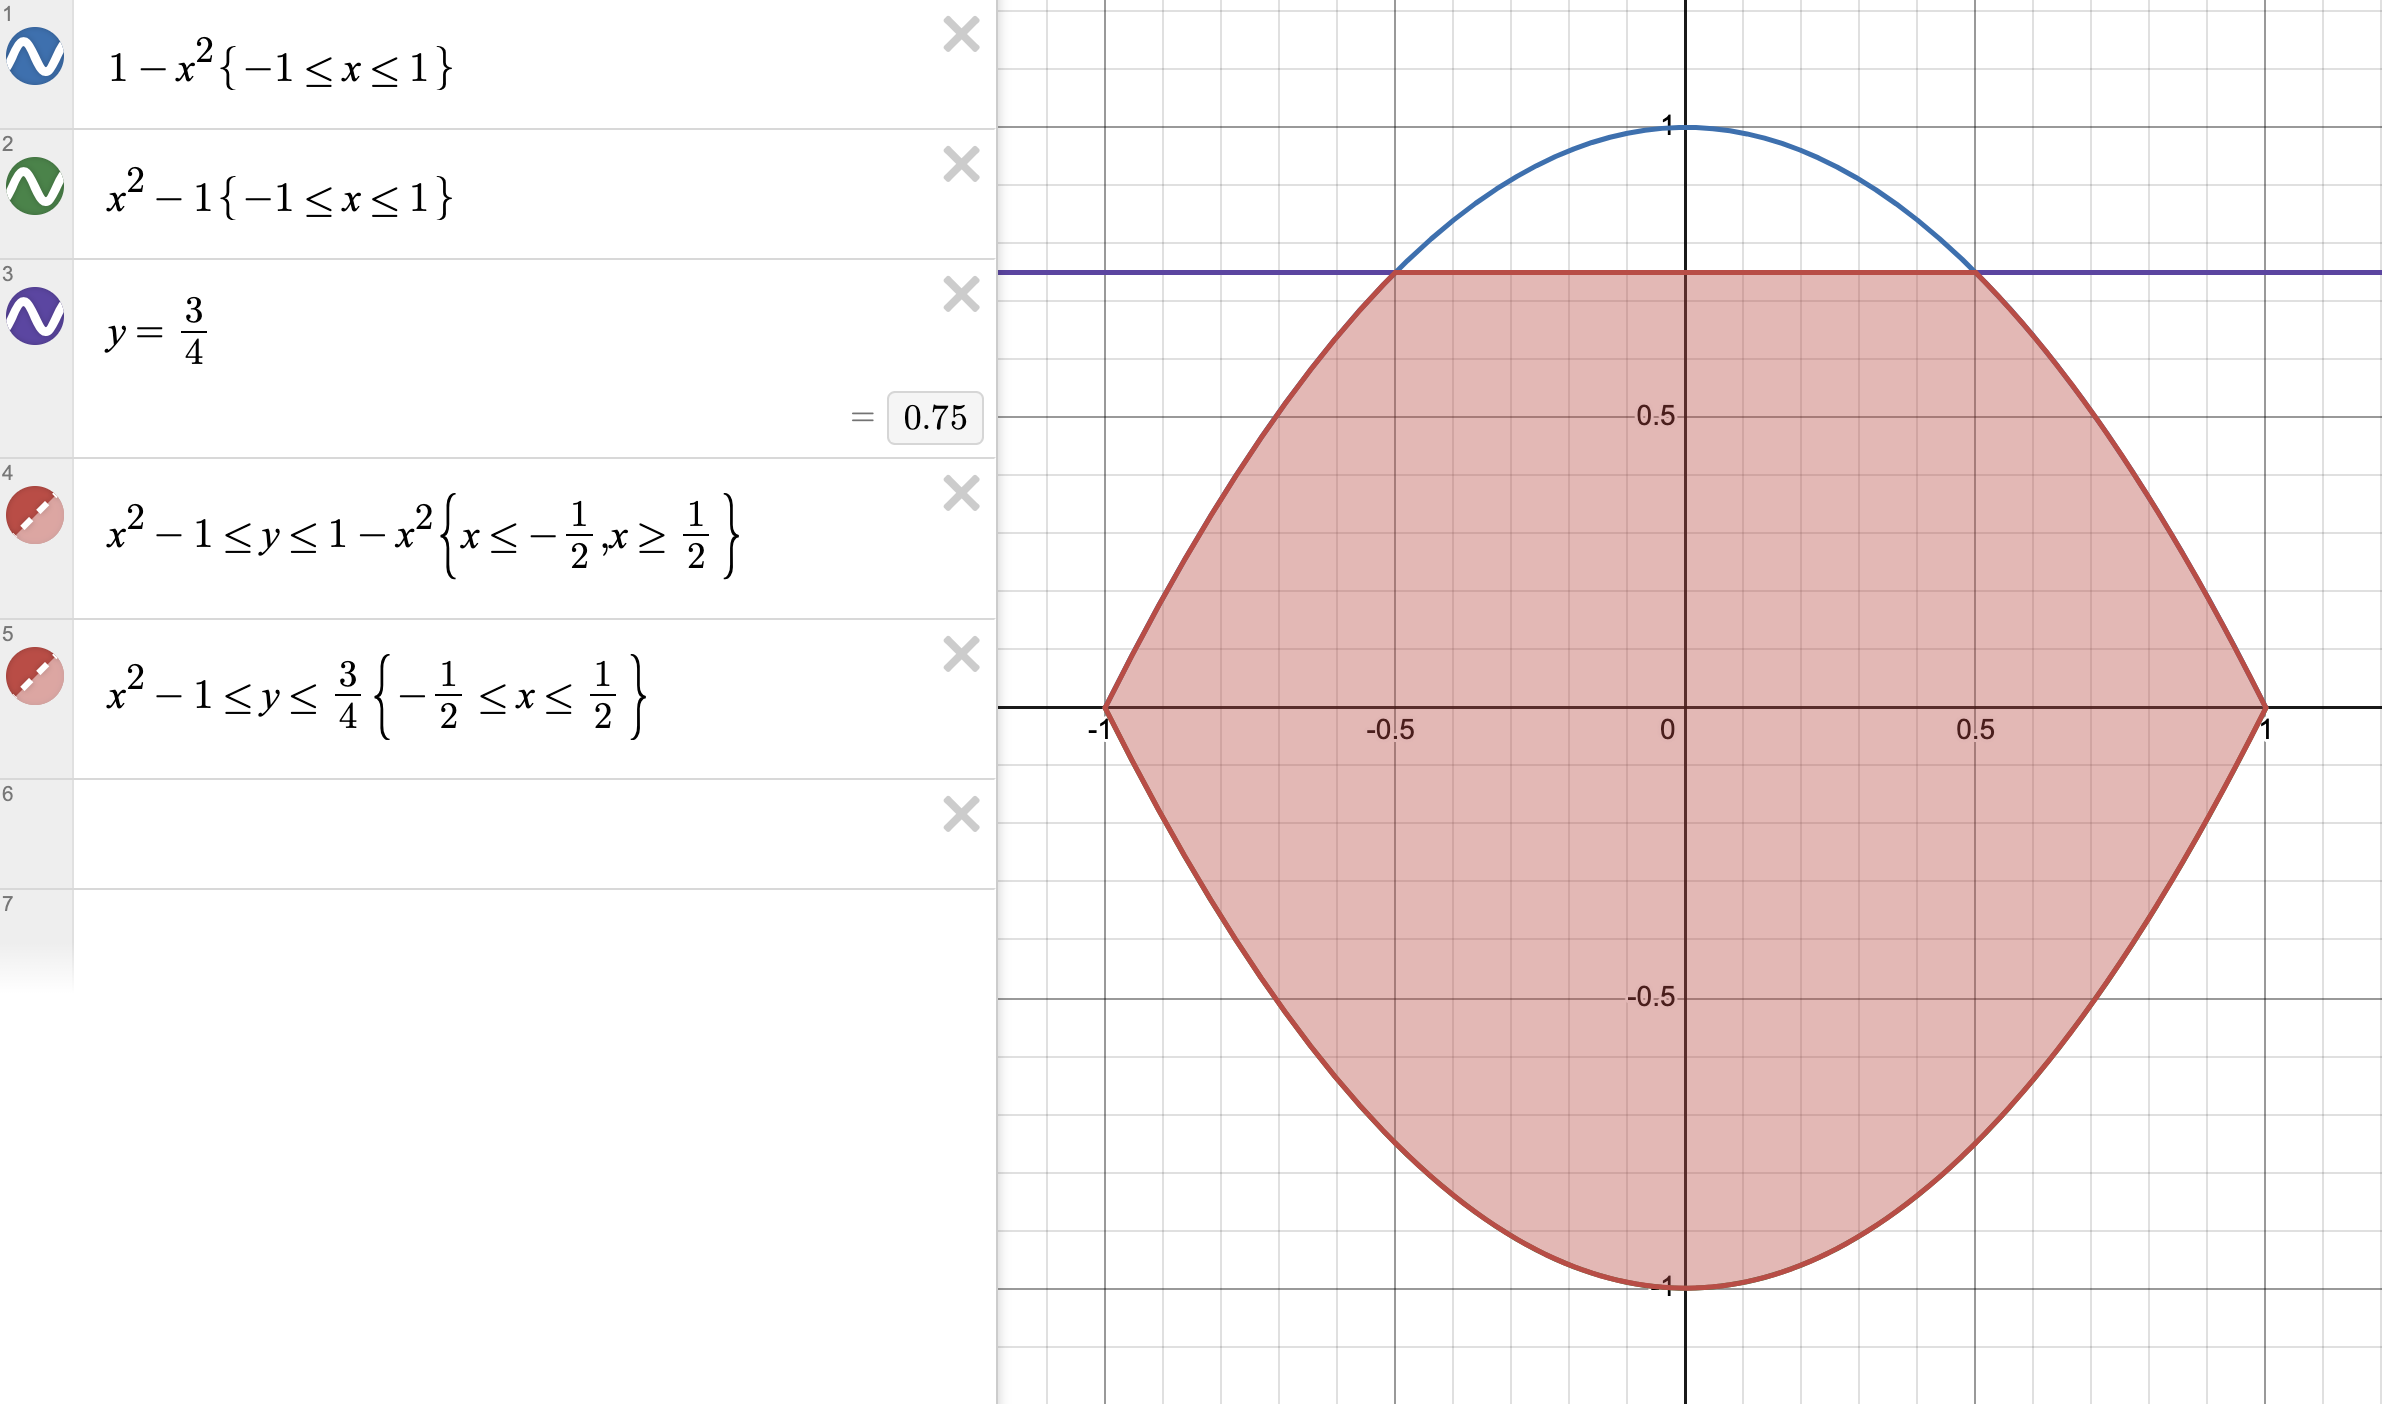
\includegraphics[width=110mm]{q4_g2.png}
    \end{figure}

    \newpage

    Which, $\PP(Y\leq \frac{3}{4})<1$, since it doesn't cover the whole region. More rigorously, given $1-x^2 = \frac{3}{4}$, we have $x^2=\frac{1}{4}$, or $x=\pm\frac{1}{2}$. Which, for $x<-\frac{1}{2}$ or $x>\frac{1}{2}$, one has $1-x^2 < \frac{3}{4}$; else for $x\in[-\frac{1}{2},\frac{1}{2}]$, one has $1-x^2\geq \frac{3}{4}$. So, the area is given as follow:
    \begin{align}
        A\left(Y\leq \frac{3}{4}\right) &= \int_{-1}^{-\frac{1}{2}}\left((1-x^2)-(x^2-1)\right)dx + \int_{-\frac{1}{2}}^{\frac{1}{2}}\left(\frac{3}{4}-(x^2-1)\right)dx + \int_{\frac{1}{2}}^{1}\left((1-x^2)-(x^2-1)\right)dx\\
        &= 2\int_{\frac{1}{2}}^{1}2(1-x^2)dx + 2\int_{0}^{\frac{1}{2}}\left(\frac{7}{4}-x^2\right)dx = 2-\frac{4}{3}x^3\bigg|_{\frac{1}{2}}^{1} + \frac{7}{4} - \frac{2}{3}x^3\bigg|_{0}^{\frac{1}{2}}\\
        &= \frac{15}{4} - \frac{7}{6} - \frac{1}{12}= \frac{5}{2}
    \end{align}
    Which, the total area bounded by the two equations are given as follow:
    \begin{align}
        A = \int_{-1}^{1}\left((1-x^2)-(x^2-1)\right)dx = 2\int_{-1}^{1}(1-x^2)dx = 4 - \frac{2}{3}x^3\bigg|_{-1}^{1} = 4-\frac{4}{3} = \frac{8}{3}
    \end{align}
    So, $\PP(Y\leq \frac{3}{4}) = A\left(Y\leq \frac{3}{4}\right)/A = \frac{5}{2}\cdot \frac{3}{8} = \frac{15}{16}<1$.

    This shows that $\PP(Y\leq \frac{3}{4}|X\leq -\frac{1}{2}) \neq \PP(Y\leq \frac{3}{4})$, hence $X,Y$ are not independent.
\end{proof}

\hfil

\hfil

\section*{5}
\begin{ques}\label{q5}
    8.Rev.21:

    Let the joint probability density function of random variables $X$ and $Y$ be given by 
    $$f(x,y)=\begin{cases}
        1 & |y|<x,\ 0<x<1\\
        0 & \text{otherwise}
    \end{cases}$$
    Show that $\EE[Y|X=x]$ is a linear function of $x$ while $\EE[X|Y=y]$ is not a linear function of $y$.
\end{ques}

\begin{proof}
    First, about $\EE[Y|X=x]$, we need to get the conditional probability density $f_{Y|X}(y|x) = \frac{f(x,y)}{f_X(x)}$. Which, for $x\leq 0$ or $x\geq 1$, since $f(x,y)=0$, one has $f_X(x) = \int_{-\infty}^{\infty}f(x,y)dy = 0$; else, for $0<x<1$, since $f(x,y)$ is $1$ if $|y|<x$ (or $-x<y<x$) and $0$ elsewhere, one gets the following for $f_X(x)$:
    \begin{align}
        f_X(x)=\int_{-\infty}^{\infty}f(x,y)dy = \int_{-x}^{x}1 dy  = 2x
    \end{align}
    So, $f_X(x) = \begin{cases}
        2x & 0<x<1\\
        0 &\text{otherwise}
    \end{cases}$. Hence, for $0<x<1$ (where $f_X(x)\neq 0$), one has $f_{Y|X}(y|x) = \frac{f(x,y)}{f_X(x)} = \begin{cases}
        \frac{1}{2x} & -x<y<x\\
        0 & \text{otherwise}
    \end{cases}$. So, the conditional expected value $\EE[Y|X=x]$ is as follow:
    \begin{align}
        \EE[Y|X=x] &= \int_{-\infty}^{\infty}y\cdot f_{Y|X}f(y|x)dy = \int_{-x}^{x}\frac{y}{2x}dy  = 0
    \end{align}
    Hence, $\EE[Y|X=x] = 0$ for all $0<x<1$, which is a linear function of $x$ on the domain.

    \hfil

    Now, about $\EE[X|Y=y]$, we need to get the conditionall probability density $f_{X|Y}(x|y) = \frac{f(x,y)}{f_Y(y)}$ instead. Which, for $y\leq -1$ or $y\geq 1$ (i.e. $|y|\geq 1$), since $f(x,y)=0$ (due to the fact that $|y|<x$ implies $x\geq 1$, which the condition for $f(x,y)=1$ is not satisfied), then $f_Y(y) = \int_{-\infty}^{\infty}f(x,y)dx = 0$.

    Now, if $-1<y< 0$, since for $f(x,y)\neq 0$, one needs $|y|<x<1$, so $-y<x<1$. Hence, the marginal probability density of $Y$ is:
    \begin{align}
        f_Y(y)=\int_{-y}^{1}f(x,y)dx = \int_{-y}^{1}1dx = 1+y
    \end{align}
    Else, if $0\leq y<1$, since for $f(x,y)\neq 0$, one needs $|y|<x<1$, so $y<x<1$. Hence, the marginal probability density of $Y$ is:
    \begin{align}
        f_Y(y) = \int_{y}^{1}f(x,y)dx = \int_{y}^{1}1 dx = 1-y
    \end{align}
    So, $f_Y(y) = \begin{cases}
        1+y & -1<y<0\\
        1-y & 0<y<1\\
        0 & \text{otherwise}
    \end{cases}$. Hence, for $|y|<1$ (where $f_Y(y)\neq 0$), one has $f_{X|Y}(x|y) = \frac{f(x,y)}{f_Y(y)} = \begin{cases}
        \frac{1}{1+y} & -1<y<0,\ -y<x<1\\
        \frac{1}{1-y} & 0\leq y<1,\ y<x<1\\
        0 & \text{otherwise}
    \end{cases}$. So, the conditional expected value $\EE[X|Y=y]$ is as follow:
    \begin{align}
        &-1<y<0\implies \EE[X|Y=y] = \int_{0}^{1}x \cdot f_{X|Y}(x|y)dx = \int_{-y}^{1}\frac{x}{1+y}dx = \frac{x^2}{2(1+y)}\bigg|_{-y}^{1} = \frac{1-y^2}{2(1+y)} = \frac{1-y}{2}\\
        &0\leq y<1\implies \EE[X|Y=y] = \int_{0}^{1}x\cdot f_{X|Y}(x|y)dx = \int_{y}^{1}\frac{x}{1-y}dx= \frac{x^2}{2(1-y)}\bigg|_{y}^{1} = \frac{1-y^2}{2(1-y)} = \frac{1+y}{2}
    \end{align}
    So, on the domain $|y|<1$, $\EE[X|Y=y] = \begin{cases}
        \frac{1+(-y)}{2} & -1<y<0\\
        \frac{1+y}{2} & 0\leq y<1
    \end{cases} = \frac{1+|y|}{2}$, which is no longer linear.
\end{proof}

\newpage

\section*{6}
\begin{ques}
    10.2.18:

    Let $X$ and $Y$ have the following joint probability density function 
    $$f(x,y)=\begin{cases}
        8xy & 0<x\leq y<1\\
        0 & \text{otherwise}
    \end{cases}$$
    \begin{itemize}
        \item[(a)] Calculate $\Var(X+Y)$.
        \item[(b)] Show that $X$ and $Y$ are not independent. Explain why this doesn't contradict Exercise 23 of Section 8.2. 
    \end{itemize}
\end{ques}
\begin{proof}
    \begin{itemize}
        \item[(a)] Given $\EE[X+Y]$ and components of $\EE[(X+Y)^2]$ as follow:
        \begin{align}
            \EE[X+Y] &= \int_{x=0}^{1}\int_{y=x}^{1}(x+y)\cdot 8xy\ dydx = \int_{x=0}^{1}\left(4x^2y^2 + \frac{8}{3}xy^3\right)\bigg|_{x}^{1}dx\\ 
            &= \int_{0}^{1}\left(\left(4x^2+\frac{8x}{3}\right) - \left(4x^4 + \frac{8x^4}{3}\right)\right)dx = \frac{4}{3}x^3 + \frac{4}{3}x^2 - \frac{4}{3}x^5\bigg|_{0}^{1}= \frac{4}{3}
        \end{align}
        \begin{align}
            \EE[X^2] &= \int_{x=0}^{1}\int_{y=x}^{1}x^2\cdot 8xy\ dy dx = \int_{x=0}^{1}4x^3y^2\bigg|_{x}^{1}dx = \int_{0}^{1}4x^3(1-x^2)dx\\ 
            &= x^4 - \frac{2}{3}x^6\bigg|_{0}^{1} = \frac{1}{3}
        \end{align}
        \begin{align}
            \EE[2XY] &= \int_{x=0}^{1}\int_{y=x}^{1}2xy \cdot 8xy\ dy dx = \int_{0}^{1}\frac{16}{3}x^2y^3\bigg|_{x}^{1}dx = \int_{0}^{1}\frac{16}{3}x^2(1-x^3)dx \\
            &= \frac{16}{9}x^3 - \frac{8}{9}x^6\bigg|_{0}^{1} = \frac{8}{9}
        \end{align}
        \begin{align}
            \EE[Y^2] &= \int_{x=0}^{1}\int_{y=x}^{1}y^2\cdot 8xy\ dydx = \int_{0}^{1}2xy^4\bigg|_{x}^{1}dx = \int_{0}^{1}2x(1-x^4)dx\\
            &= x^2 - \frac{1}{3}x^6\bigg|_{0}^{1} = \frac{2}{3}
        \end{align}
        Hence, $\EE[(X+Y)^2]= \EE[X^2]+\EE[2XY]+\EE[Y^2] = \frac{17}{9}$. So, $\Var(X+Y) = \EE[(X+Y)^2]-\EE[X+Y]^2 = \frac{17}{9}- \frac{16}{9}=\frac{1}{9}$.
        
        \hfil

        \item[(b)] Consider the probability $\PP(Y\leq \frac{1}{2})$ and $\PP(Y\leq \frac{1}{2}|X\leq \frac{1}{2}) = \frac{Y\leq \frac{1}{2},X\leq \frac{1}{2}}{\PP(X\leq \frac{1}{2})}$: 
        \begin{align}
            \PP\left(Y\leq \frac{1}{2}\right) = \int_{y=0}^{\frac{1}{2}}\int_{x=0}^{y}8xy\ dx dy = \int_{0}^{\frac{1}{2}}4yx^2\bigg|_{0}^{\frac{1}{2}}dy = \int_{0}^{\frac{1}{2}}y\ dy = \frac{1}{8}
        \end{align}
        \begin{align}
            \PP\left(X\leq \frac{1}{2}\right) &= \int_{x=0}^{\frac{1}{2}}\int_{y=x}^{1}8xy\ dydx = \int_{0}^{\frac{1}{2}}4xy^2\bigg|_{x}^{1}dx = \int_{0}^{\frac{1}{2}}4x(1-x^2)dx \\
            &=  2x^2-x^4\bigg|_{0}^{\frac{1}{2}} = \frac{1}{2} - \frac{1}{16} = \frac{7}{16}
        \end{align}
        \begin{align}
            \PP\left(Y\leq \frac{1}{2},X\leq \frac{1}{2}\right)&=\int_{x=0}^{\frac{1}{2}}\int_{y=x}^{\frac{1}{2}}8xy\ dydx = \int_{0}^{1}4xy^2\bigg|_{x}^{\frac{1}{2}}dx = \int_{0}^{\frac{1}{2}}4x\left(\frac{1}{4}-x^2\right)dx\\
            &= \int_{0}^{\frac{1}{2}}(x-4x^3)dx = \frac{1}{2}x^2-x^4\bigg|_{0}^{\frac{1}{2}} = \frac{1}{8}-\frac{1}{16} = \frac{1}{16}
        \end{align}
        Hence, $\PP(Y\leq\frac{1}{2}|X\leq \frac{1}{2})=\frac{1/16}{7/16} = \frac{1}{7}$, while $\PP(Y\leq \frac{1}{2})=\frac{1}{8}\neq \PP(Y\leq \frac{1}{2}|X\leq \frac{1}{2})$, this shows that $X,Y$ are not independent.

        This doesn't violate the given relation in 8.2 Exercise 23, because here the separation of the function $f(x,y)$ still has $x$ being dependent on $y$, which there doesn't exist a function $g(x), h(y)$ such that the multiplication is $f(x,y)$ (since one must has boundary condition dependent on the other).
    \end{itemize}
\end{proof}
\begin{comment}
\section*{6}
\begin{ques}\label{q6}
    10.2.18:

    For random variables $X$ and $Y$, show that 
    $$\Cov(X+Y,X-Y) = \Var(X)-\Var(Y)$$
\end{ques}

\begin{proof}
    Recall that $\Cov(U,V) = \EE[U V] - \EE[U]\cdot \EE[V]$. Then, for $U=X+Y$ and $V=X-Y$, one has the following:
    \begin{align}
        &\EE[U V] = \EE[(X+Y)(X-Y)] = \EE[X^2-Y^2] = \EE[X^2]-\EE[Y^2]\\
        &\EE[U]\EE[V] = \EE[X+Y]\cdot\EE[X-Y] = \left(\EE[X]+\EE[Y]\right)\left(\EE[X]-\EE[Y]\right) = \EE[X]^2 - \EE[Y]^2
    \end{align}
    Hence, we get:
    \begin{align}
        \Cov(X+Y,X-Y) &= \EE[UV]-\EE[U]\EE[V] = (\EE[X^2]-\EE[Y^2]) - (\EE[X]^2-\EE[Y]^2)\\ 
        &= (\EE[X^2]-\EE[X]^2) - (\EE[Y^2]-\EE[Y]^2) = \Var(X)-\Var(Y)
    \end{align}
\end{proof}
\end{comment}
\hfil

\hfil

\section*{7}
\begin{ques}\label{q7}
    10.2.25:

    A fair die is thrown $n$ times. What is the covariance of the number of $1$'s and the number of $6$'s obtained?
\end{ques}

\begin{proof}
    Let $X_i$ and $Y_i$ represents the the indicator for the $i^\text{th}$ throw being $1$ or $6$ respectively, then each $X_i, Y_i \sim \Ber(\frac{1}{6})$ (since there is a $\frac{1}{6}$ chance of being the desired number). Which, define $X=\sum_{i=1}^{n}X_i$ and $Y=\sum_{j=1}^{n}Y_j$, $X,Y$ represent the number of $1$'s and $6$'s, respectively.

    \hfil

    Now, using the bilinearity of covariance, we have:
    \begin{align}
        \Cov(X,Y) &= \sum_{i=1}^{n}\sum_{j=1}^{n}\Cov(X_i, Y_j) = \sum_{i=1}^{n}\sum_{j=1}^{n}\left(\EE[X_i Y_j] - \EE[X_i]\EE[Y_j]\right)\\ 
        &= \sum_{i=1}^{n}\left(\EE[X_i Y_i]-\frac{1}{36}\right) + \sum_{i\neq j}\left(\EE[X_i]\EE[Y_j] - \EE[X_i]\EE[Y_j]\right)\\
        &= \sum_{i=1}^{n}\left(0-\frac{1}{36}\right) = -\frac{n}{36}
    \end{align}
    (Note: if $i\neq j$, since each row is independent, one has $X_i, Y_j$ being independent, hence $\EE[X_iY_j]=\EE[X_i]\EE[Y_j]$; And, since $X_i$ and $Y_i$ cannot both be $1$ due to the fact that rolling a number resulting in not rolling the other number, so $X_i Y_i=0$ regardless).
    \begin{comment}
    First, let $X, Y$ be the random variable of the number of $1$'s and $6$'s within this $n$ throws respectively. Then, both $X,Y\sim \Bin(n, \frac{1}{6})$ (since each throw has a $\frac{1}{6}$ chance of getting 1, or getting 6 respectively, and there are $n$ independent throws). Hence, one has $\EE[X]=\EE[Y] = n p = \frac{n}{6}$, and $\Var(X) =\Var(Y) = \frac{5n}{36}$.

    \hfil
    
    Now, to get $\EE[X Y]$, since another restriction one has is $X+Y \leq n$ (since $X,Y$ cannot represent the same collection of throws, because each throw only corresponds to one output; and, there's total of $n$ throws only). So, using conditional probability, one has $\PP(X=i, Y=j) = \PP(Y=j|X=i)\PP(X=i)$, whre $\PP(X=i) = \begin{pmatrix}
        n\\i
    \end{pmatrix}\left(\frac{1}{6}\right)^i\left(\frac{5}{6}\right)^{n-i}$, and one requires $i+j\leq n$, so if $i+j>n$, one has $\PP(X=i,Y=j)=0$. Hence, it suffices to understand the distribution of $(Y|X=i)$. 

    If $X=i$, then $Y\leq n-i$; also, since each throw of the fair die within these $n-i$ throws can only have $5$ possible outcomes (since already excluded the possibility that the die gets a $1$, because all the thorws with $1$ are collected by random variable $X$), and each outcome is equally possible to happen, then each throw has a $\frac{1}{5}$ chance of getting outcome $6$. Hence, one has $(Y|X=i) \sim \Bin(n-i, \frac{1}{5})$, showing $\PP(Y=j|X=i) = \begin{pmatrix}
        n-i\\j
    \end{pmatrix}\left(\frac{1}{5}\right)^j\left(\frac{4}{5}\right)^{n-i-j}$, and $\EE[Y|X=i] = \frac{n-i}{5}$.

    Finally, this gives the following expected value:
    \begin{align}
        \EE[XY]&= \sum_{i=0}^{n}\sum_{j=0}^{n}(i j)\cdot \PP(X=i,Y=j) = \sum_{i=0}^{n}\sum_{j=0}^{n-i}(i j)\cdot \PP(Y=j|X=i)\PP(X=i)\\
        &= \sum_{i=0}^{n}i\cdot \PP(X=i)\left(\sum_{j=0}^{n-i}j\cdot \PP(Y=j|X=i)\right)= \sum_{i=0}^{n}i\cdot\EE[Y|X=i]\cdot \PP(X=i)\\
        &= \sum_{i=0}^{n}i \cdot \frac{n-i}{5}\cdot \PP(X=i) = \frac{n}{5}\cdot\EE[X] - \frac{1}{5}\cdot \EE[X^2] = \frac{n}{5}\cdot\EE[X] - \frac{1}{5}\left(\Var(X) + \EE[X]^2\right)
    \end{align}
    Hence, plugin the values, one has:
    \begin{align}
        \EE[XY]&=\frac{n}{5}\cdot\frac{n}{6} - \frac{1}{5}\left(\frac{5n}{36} + \frac{n^2}{36}\right) = n^2\left(\frac{1}{30}-\frac{1}{36}\right) - \frac{n}{36} = \frac{n^2 - 5n}{180}
    \end{align}
    So, the covariance is given as follow:
    \begin{align}
        \Cov(X,Y)=\EE[XY]-\EE[X]\EE[Y]=\frac{n^2-5n}{180} - \frac{n^2}{36} = -\frac{4n^2+5n}{180}
    \end{align}
    \end{comment}
    
\end{proof}

\newpage

\section*{8}
\begin{ques}\label{q8}
    10.4.9:

    Prove that, for a Poisson random variable $N$, if the parameter $\lambda$ is not fixed and is itself an exponential random variable with parameter $1$, then 
    $$\PP(N=i) = \left(\frac{1}{2}\right)^{i+1}$$
\end{ques}

\begin{proof}
    Let If fixing the parameter $\lambda=t$, one had $N \sim \Poi(t)$, so one has $\PP(N=i\ |\ \lambda =t) = e^{-t}\frac{t^i}{i!}$. However, since $\lambda \sim \Exp(1)$, one has its probability density $f_\lambda(t) = e^{-t}$. So, using the Law of Total Probability, we have the following:
    \begin{align}
        \PP(N=i) &= \int_{0}^{\infty}\PP(N=i\ |\ \lambda =t)\cdot f_\lambda (t)dt = \int_{0}^{\infty}\left(e^{-t}\frac{t^i}{i!}\right)e^{-t}dt = \frac{1}{i!}\int_{0}^{\infty}t^i e^{-2t}dt\\
        &= \frac{1}{2\cdot i!}\int_{0}^{\infty}\left(\frac{u}{2}\right)^i e^{-u}du = \frac{1}{i!}\left(\frac{1}{2}\right)^{i+1}\int_{0}^{\infty}u^i e^{-u}du = \frac{1}{i!}\left(\frac{1}{2}\right)^{i+1}\Gamma(i+1) = \left(\frac{1}{2}\right)^{i+1}
    \end{align}
\end{proof}

\hfil

\hfil

\section*{9}
\begin{ques}\label{q9}
    10.4.13:

    During an academic year, the admissions office of a small college receives student applications at a Poisson rate of $5$ per day. It is a policy of this college to double its student recruitment efforts if no applications arrive for two consecutive business days. Find the expected number of business days until a time when the college needs to double its recruitment efforts. Do the admission officers need to worry about this policy at all?

    Hint: Let $X_1$ be the time until the first application arrives. Let $X_2$ be the time between the first and second applications, and so forth. Let $N$ be the first integer for which 
    $$X_1\leq 2,\quad X_2\leq 2,\quad \cdots,\quad X_N\leq 2,\quad X_{N+1}\geq 2 $$
    The time that the admissions office has to wait before doubling its student recruitment efforts is $S_{N+1} = X_1+X_2+...+X_{N+1}$. Find $S_{N+1}$ by conditioning on $N$.
\end{ques}

\begin{proof}
    Recall that given number of applications happening with rate $\Poi(5t)$ (where $t$ is the duration of the days being viewed), then let $X_n$ denotes the time between $n-1$ to $n$ arrival, one has $X_n \sim \Exp(5)$ (these are based on class notes).

    Then, if fix the number of arrivals $N$ with $n\leq N$ implies $X_n\leq 2$, one has the following conditional probability density:
    \begin{align}
        \forall 0<x\leq 2,\quad f_{X_n|X_n\leq 2}(x) = \frac{5e^{-5x}}{\int_{0}^{2}5e^{-5t}dt} = \frac{5e^{-5x}}{1-e^{-10}}
    \end{align}
    As a result, the expected value of $X_n$ is as follow:
    \begin{align}
        \EE[X_n|X_n\leq 2]&=\int_{0}^{2}x\cdot f_{X_n|X_n\leq 2}(x)dx = \int_{0}^{2}\frac{5xe^{-x}}{1-e^{-10}}dx = \frac{1}{1-e^{-10}}\left(-xe^{-5x}\bigg|_{0}^{2} + \int_{0}^{2}e^{-5x}dx\right)\\
        &= \frac{1}{1-e^{-10}}\left(-2e^{-10}-\frac{e^{-5x}}{5}\bigg|_{0}^{2}\right) = \frac{1}{5(1-e^{-10})}\left(-10e^{-10}+1-e^{-10}\right)\\
        &= \frac{1-9e^{-10}}{5(1-e^{-10})}
    \end{align}
    Now, for $X_{N+1}$, given $X_{N+1}\geq 2$, one has the following conitional probability density:
    \begin{align}
        \forall 2\leq x, \quad f_{X_{N+1}|X_{N+1}\geq 2}(x) = \frac{5e^{-5x}}{\int_{2}^{\infty}5e^{-5t}dt} = \frac{5e^{-5x}}{e^{-10}}
    \end{align}
    As a result, the expected value of $X_{N+1}$ is as follow:
    \begin{align}
        \EE[X_{N+1}|X_{N+1}\geq 2] &= \int_{2}^{\infty}x\cdot f_{X_{N+1}|X_{N+1}\geq 2}(x)dx=\int_{2}^{\infty}\frac{5xe^{-5x}}{e^{-10}}dx = e^{10}\left(-xe^{-5x}\bigg|_{2}^{\infty} + \int_{2}^{\infty}e^{-5x}dx\right)\\
        &= e^{10}\left(2e^{-10} + \frac{e^{-10}}{5}\right) = \frac{11}{5}
    \end{align}
    Hence, as a result, we get $\EE[S_{N+1}] = \EE[X_1]+...+\EE[X_N]+\EE[X_{N+1}] = \frac{N(1-9e^{-10})}{5(1-e^{-10})} + \frac{11}{5}$.

    \hfil

    Now, if talking about the condition on $N$, since it needs the first $N$ arrivals to have $X_n\leq 2$, which each independently has probability of $\PP(X_n\leq 2) = \int_{0}^{2}5e^{-5t}dt = 1-e^{-10}$; while for the $N+1$ arrival, one needs $X_{N+1}\geq 2$, so $\PP(X_{N+1}\geq 2) = \int_{2}^{\infty}5e^{-5t}dt = e^{-10}$. Hence, the probability that case for $N$ happens, is $\PP(N)=(1-e^{-10})^N \cdot e^{-10}$. 

    As a result, the expected value of $S$ is provided as follow:
    \begin{align}
        \EE[S] &= \sum_{N=0}^{\infty}\EE[S_{N+1}]\cdot\PP(N) = \sum_{N=0}^{\infty}\left(\frac{N(1-9e^{-10})}{5(1-e^{-10})}+\frac{11}{5}\right)\cdot (1-e^{-10})^N\cdot e^{-10}\\
        &= \frac{11}{5e^{10}}\cdot\frac{1}{1-(1-e^{-10})} + \frac{1-9e^{-10}}{5(1-e^{-10})}\sum_{N=0}^{\infty}N(1-e^{-10})^N\cdot e^{-10}\\
        &= \frac{11}{5} + \frac{1-9e^{-10}}{5(1-9e^{-10})}\cdot\frac{(1-e^{-10})}{e^{-20}}\cdot e^{-10} = \frac{11}{5}+\frac{e^{10}-1}{5} = 2+\frac{e^{10}}{5}\approx 4407.2932
    \end{align}
    Which, in practical this number is large enough so that in general it's not part of the worry.
\end{proof}

\newpage

\section*{10}
\begin{ques}\label{q10}
    The number of espresso shots that the Arbor coffee shop uses per order has a $\Bin(4,0.3)$ distribution. Suppose that $20\%$ of the customers are professors (independent of everything else) and the rest are students. Find the mean and the variance of the number of espresso shots that would be pulled until the next professor arrives.
\end{ques}

\begin{proof}
    Here, assume for each order there are $4$ shots, each independently has a $0.3$ probability of being espresso (to interpret why each order has distribution $\Bin(4,0.3)$). Which, if let $X_i$ represents the number of espresso in the $i^\text{th}$ order, one has $X_i = X \sim \Bin(4,0.3)$. Which, $\EE[X] = 4\cdot 0.3 = 1.2$, and $\Var(X) = np(1-p) = 4\cdot 0.3\cdot 0.7 = 0.84$.

    Now, let $N$ represents the random variable of number of customers before the next professor arrives, since for each customer there is a $0.2$ chance that a professor arrives (and a $0.8$ chance that is not a professor), then for any $n \in \NN$, one has the probability of $N=n$ given as $\PP(N=n) = (0.8)^n\cdot (0.2)$ (since we need $n$ consecutive students, while the $(n+1)^\text{th}$ customer is a professor). Hence, $N$ is of a geometric distribution, with $\EE[N] = \sum_{n=0}^{\infty}n\cdot (0.8)^n(0.2) = 4$, and $\EE[(N+1)(N+2)]$ is given as follow (using the identity $\sum_{n=0}^\infty (n+1)(n+2)x^n = \frac{2}{(1-x)^3}$ for $|x|<1$):
    \begin{align}
        \EE[N^2]+3\EE[N]+2 &= \EE[N^2+3N+2]=\EE[(N+1)(N+2)] = \sum_{n=0}^{\infty}(n+1)(n+2)\cdot (0.8)^n\cdot 0.2\\
        &= 0.2\cdot \frac{2}{(1-0.8)^3} = 0.2\cdot \frac{2}{0.2^3} = \frac{2}{0.2^2} = 50
    \end{align}
    Which, $\EE[N^2]+3\EE[N]+2 = 50$, with $\EE[N] = 4$, one has $\EE[N^2] = 36$. So, $\Var(N) = \EE[N^2]-\EE[N]^2 = 36-16=20$.

    \hfil

    Now, since $N$ is independent from each $X_i$, with $N=n$ fixed, the number of espresso shots ordered is recorded by random sum $S=\sum_{i=1}^n X_i$ (where each $X_i$ are identical), then using the formulas, we have the following:
    \begin{align}
        \EE[S] = \EE[X]\cdot \EE[N] = 1.2\cdot 4 = 4.8
    \end{align}
    \begin{align}
        \Var(S) = \Var(X)\cdot \EE[N]+\EE[X]^2\cdot \Var(N) = 0.84\cdot 4+1.2^2\cdot 20 = 32.16
    \end{align}
\end{proof}

\end{document}